\chapter[Applications of the Formula of Jensen and...]{Applications of the Formula of Jensen and
 Carleman \\ to quasi-analytic Classes $D$ and $I (\alpha)$}\label{chap21}%chap 21 

\section{Principle of the method}\label{chap21:sec1}%sec 1

We\pageoriginale give here an alternative method for obtaining conditions of
quasi-analyticity. This method is applicable to bounded mean-periodic
functions (for quasi-analyticity $I(\alpha)$ and for mean periodic
functions belonging to a class $C\{M_n\}$ (for quasi-analyticity
$D$). Moreover, it is easily seen that the method can be applied to
those classes of bounded functions on the real line whose Carleman
transforms (in the classical sense) are meromorphic, either on the
whole plane or at the right (left) of the imaginary axis (for example,
almost periodic functions whose spectrum have no finite point of
accumulation on the line (resp. on a half line ) ). 

Following a method of $B$. Levin, we take $I (\alpha) = e^{- \alpha r
 (\alpha)} $ where $r (\alpha)$ is a decreasing function of $\alpha$
which is $\infty$ on $[0, \alpha_\infty]$ and continuous with values
from $\infty$ to $r_o$ on $(\alpha_\infty, \alpha_o ], 0 \le
 \alpha_\infty < \alpha_o$. We denote $l_g/\alpha (r)$ the inverse
 function, defined on $[ r_o, \infty)$, such that $\alpha (\infty) =
 \alpha_\infty$. 

Let now $\int^\alpha_o | f | \le I (\alpha) ~ (0 < \alpha < \alpha_o)
$; if $\alpha_\infty \neq 0$, this means $f = 0$ on $[0,
 \alpha_\infty]$. Let $F(w)$ be the Carleman transform of $f
$(Lect. $6, \S 3)$. 
\begin{align*}
 F(w) & = \int\limits^o_{- \infty} f(x) e^{ixw} dx \text { for } ~ v > 0\\
 F(w) & = - \int\limits^{\infty}_o f(x) e^{-xw } dx \quad \text {for } ~ v < 0.
\end{align*}

We\pageoriginale have the following majorizations:
\begin{align*}
 |F(w)| &= | \int\limits_o^\infty ~ f(x) ~ e^{-ixw} ~ dx | ~ \le ~
 |~ \int\limits_o^\alpha ~ | ~ + ~ | ~ \int\limits_\alpha^\infty ~ |
 \\ 
 &\le ~ I(\alpha) + K \frac{e^{-\alpha | v |}}{| v |} ~ v < 0 \\
 &| ~ F(w) ~ | ~ \le \int\limits_{-\infty}^o ~ | ~ f(x) ~ | ~ e^{xv}
 |~ dx ~ < \frac{K}{| V |}, ~ v > 0. 
\end{align*}
\begin{figure}[H]
 \centerline{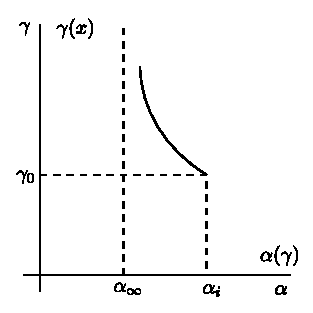
\includegraphics{vol15-figures/fig15-22.eps}}
\end{figure}

For a given $w$ we can choose $\alpha$ as we want and we take $\alpha
= \alpha (|v|)$, $| v | = r(\alpha)$. Thus the above majorization for $v
< 0$ reduces to the following one: 
$$
| F(w) | < \left(1 + \frac{K}{|v|}\right) ~ e^{-\alpha r(\alpha)} ~ \le ~ \left(1+
\frac{K}{|v|}\right) ~ e^{- | v | \alpha(|w|)}. 
$$

This relation permits us to have the following lemma:

\setcounter{lem}{0}
\begin{lem}\label{chap21:sec1:lem1}% lemma 1
 The set of bounded functions in $\mathscr{C}_{\Lambda} \neq
 \mathscr{C}$ is an $I(\alpha)$ quasi-analytic class, with
 $I(\alpha) = e^{-\alpha r(\alpha)}$as soon as the following relation
 is satisfied: 
 \begin{equation*}
 \left.
 \begin{aligned}
  \log | F(w) | < - \log | v |, v > 0 ~ (w = u+iv = re^{i\theta})&
  \quad \\
  \log | F(w) | < - \log \frac{|v|}{|1+v|} - | v | \alpha (r), v <
  0\\
  F(w)~~ \text{\em meromorphic with simple poles at } \Lambda.&
 \end{aligned}
 \right \}
 \Rightarrow F \equiv 0
 \end{equation*}
\end{lem}

Let now $f \in C\{M_n\}\cap
\mathscr{C}_{\Lambda},\mathscr{C}_{\Gamma}\neq \mathscr{C}$ and
$f^{(n)}(0)=0$ for every $n$. 

Then $F(w)$ satisfies the following relations:
\begin{align*}
 F(w) & = \int\limits_{-\infty}^o ~ f^{(n)} ~ (x)
 \frac{e^{-ixw}}{(iw)^n} ~ dx ~~ v > 0\\ 
 | F(w)| &< \frac{K ~ M_n}{|w|^n} ~ \int\limits_{-\infty}^o ~
 e^{vx} ~ dx = \frac{K ~ M_n}{|v| ~r^n} ~ ~v > 0\\ 
 | F(w)| & < \frac{K ~ M_n}{| v | r^n} ~ \qquad v < 0
\end{align*}

We have seen in Lecture $7$ (since $f$ is bounded) that $F(w)$ is a
meromorphic function with real simple poles at $\Lambda$ and from the
above inequalities we have $|F(w) | < \inf_{n} \dfrac{K ~ M_n}{|v| ~
 r^n}$. 

Thus\pageoriginale we have the following Lemma: 

\begin{lem}\label{chap21:sec1:lem2}% lemma 2
 The class $\mathscr{C}_\Lambda \cap C\{M_n \}, \mathscr{C}_\Lambda
 \neq \mathscr{C}$ is a $D$-quasi-analytic class as soon as the
 following relation is satisfied: 
 \begin{equation*}
 \left.
 \begin{aligned}
  &F(w) \text{ if meromorphic with simple poles at }\Lambda\\
  &\log | F(w) | < - \log | v | - S(r) \\
  &\text{ with } S(r) = \max_n (n \log r - \log M_n) 
 \end{aligned}
 \right \}
 \Rightarrow F \equiv 0
 \end{equation*}
\end{lem}

\section{Application of Jensen's and Carleman's formulae}\label{chap21:sec2}%Sec 2

\textbf{Application of Jensen's formula:} Here we assume $\Lambda =
\{\pm \lambda_n \}$. Definitions of $n(r),\bar{D}(r),\bar{D}^.$ are
given in Lect. 10. \S \ref{chap10:sec1}. 

We suppose that $F(w)$ satisfies the majorizations of Lemma
\ref{chap21:sec1:lem1}  and
that $F(w) \nequiv 0$. First, Jensen's formula gives the following
majorization: (Lecture 10.\S \ref{chap10:sec2}) 
$$
-2 ~ \int\limits_o^r ~ \frac{n(t)}{t} ~ dt \le \frac{1}{2\pi}
\int\limits_o^{2\pi} ~ \log | F(re^{i\theta}) ~ | ~ d\theta - \log ~ |
~F(0) ~ | 
$$

Division of $F(w)$ by $w^p$ will not alter the conditions of Lemma
\ref{chap21:sec1:lem1} 
and so we can take $F(0) \neq 0$. Using the majorizations of Lemma
\ref{chap21:sec1:lem1} 
in the above inequality, we have 
$$
-2 ~ r ~ \bar{D} ~ (r) < - \frac{1}{\pi} ~ r\alpha(r) - \frac{1}{2}
~ \log ~ r + 0(1) 
$$
and so $\alpha (r) < 2 \pi\bar{D}(r)$ for sufficiently large $r$.

This relation gives us the following theorem:

\setcounter{theorem}{0}
\begin{theorem}\label{chap21:sec2:thm1}% theorem 1
 The set of bounded functions of $\mathscr{C}_\Lambda \neq
 \mathscr{C}$ is an $I(\alpha)$ quasi-analytic class, with $I(\alpha)
 = e^{-\alpha r(\alpha)}$ as soon as $\alpha (r) \ge 2\pi\bar{D}(r)$
 for an infinity of values of $r \rightarrow \infty$. 
\end{theorem}

\begin{remarks*}% remarks:
 \begin{enumerate}[1)]
 \item If\pageoriginale $\alpha(\infty) > 2 \pi \bar{D}$, the above theorem gives
 that the set of bounded functions of $\mathscr{C}_\Lambda \neq
 \mathscr{C}$ is a quasi-analytic class I. $| I | = 1$, whenever $1
 > 2\pi\bar{D}$.. This result is contained in Levinson's theorem
 (Lecture 19.\S  \ref{chap19:sec1}). 
 \item If $\bar{D}(r) \le \bar{D}$. for an infinity of values of $r
 \rightarrow \infty$ it is sufficient to have $\alpha (\infty) =
 2\pi\bar{D}$. to apply the above theorem and thus, in this case,
 we get a precision of Levinson's theorem. 
 \item The above Remark $(2)$ applies to the case of odd integers
 where we have $\bar{D}. = \dfrac{1}{2}$, then also the case of
 even integers. But if we add $\pm 1 $ to $\Lambda$ the result
 ceases to apply. Indeed, there exists a function $f(x) = \sin x +
 \sum\limits_{- \infty}^{\infty} ~C_n ~ e^{2\sin x}$ which
 vanishes on $[0,\pi],f(x) \nequiv 0$. Adding $\{\pm 1 \}$ to
 $\Lambda$, we add $\dfrac{\log r}{r}$ to $\bar{D}(r)$. Thus we
 cannot replace $\bar{D}(r)$ by $\bar{D}(r) + \dfrac{\log r}{r}$ in
 the above theorem. In this sense the above theorem is a precise
 one for sequences $\Lambda$ whose distribution is nearly the same
 as that of integers. 
 \begin{figure}[H]
  \centerline{\includegraphics{vol15-figures/fig15-23.eps}}
 \end{figure}
 \end{enumerate}
\end{remarks*}

Let now $F(w)$ satisfy the conditions of Lemma \ref{chap14:lem2} and let us see what
happens when we suppose $F(w) \nequiv 0$. Applying Jensen's formula and
using the conditions of Lemma \ref{chap14:lem2}, we obtain, as before, the following
inequality: 
$$
\displaylines{\hfill 
 - 2 ~ r ~ \bar{D}(r) < - S(r) - \log ~ r + 0(1)\hfill \cr
 \text{where}\hfill 
 S(r) = \max_n ~ (n \log r - \log M_n).\hfill \cr
 \text{As}\hfill 
 r ~ \bar{D}(r) = N(r) \log ~ r - \int\limits_o^r \frac{dN(t)}{t} =
 \log \frac{r^n}{\lambda_1 \cdots \lambda_n} \hfill }
$$
if\pageoriginale $\lambda_n < r < \lambda{n+1}$, the last inequality can be written
$$
\max_n \frac{r^{2n+1}}{\lambda_1^2 \cdots \lambda^2_n} > K ~ \max
\frac{r^{2n+1}}{M_{2n+1}} \quad (K > 0). 
$$

Using the lemma stated at the end of last lecture, the above
inequality $M_{2n+1} > K | \lambda^2_1 \cdots \lambda^2_n | $ where
$K$ is a constant. Thus in order to have $F(w) \equiv 0$ it is
sufficient to have the reverse inequality for an infinity of values of
n, which gives the following theorem: 

\begin{theorem}\label{chap21:sec2:thm2}% theorem 2
 $\mathscr{C}_\Lambda \cap C \{M_n \}$ is a $D$ -quasi-analytic
  class as soon as the following condition is satisfied:
  $$
  \lim\inf_{n \rightarrow \infty} \frac{M_{2n+1}}{ \lambda^2_1
  \cdots \lambda^2_n} = 0. 
  $$
\end{theorem}

\begin{remark*}% remark
 The above condition is simpler and more precise than the condition of
 $D$ - quasi-analyticity obtained in the last lecture. However, this
 condition is applicable only when $\Lambda$ is real and it involves
 $C\{ M_n\}$ instead of $C_I \{M_n \}$. But the latter inconvenience
 can be suppressed whenever $\triangle = 0$, by the use of the
 theorem of continuation of Lecture \ref{chap17}. 
\end{remark*}

Using a result proved in the next lecture, we can obtain that the above
condition is also necessary for $D$-quasi-analyticity, when $\Lambda$
is sufficiently lacunary. 

\noindent
\textbf{Application of Carleman's formula:} We assume now nothing
about the negative part of $\Lambda$; the functions $n^+(r),D^+(r)$
are related to the positive part of $\Lambda$. 

Suppose $F(w)$ satisfies the condition of Lemma \ref{chap14:lem7} and let $F(w)
\nequiv 0$. The application of Carleman's formula in the right
half-plane gives\pageoriginale
$$
\int\limits^r (1/t - t/r^2) ~ dn^+ (t) > \frac{1}{2\pi} ~
\int\limits^r ~ (1/v^2 - 1/r^2) v \alpha (v) ~ dv + 0(1). 
$$

Now, if $D^+(r)$ is bounded, integrating by parts, this reduces $\infty$:
$$
\int\limits^r \frac{2\pi ~ D^+(t) - \alpha (t)}{t} ~ dt > 0(1).
$$

Thus we have the following theorem:

\begin{theorem}\label{chap21:sec2:thm3}% theorem 3
 The class of bounded functions of $\mathscr{C}_\Lambda \neq
 \mathscr{C}$ is an $I (\alpha)$ quasi-analytic class, with
 $I(\alpha) = e^{-\alpha r(\alpha)}$ when $D^{+.} < \infty$ and 
 $$
 \lim\sup_{r\rightarrow \infty} ~ \int\limits^r ~ \frac{\alpha(t) -
 2\pi D^+(t)}{t} ~ dt = \infty. 
 $$
\end{theorem}

Suppose now that $F(w)$ satisfies the conditions of Lemma \ref{chap14:lem2} and
$F(w) \nequiv 0$. Set $w' = ie^{-i\pi a} w^a$, with $\dfrac{1}{2} \le
a \le 1$. We take $F_1(w') = F(w).F_1(w')$ is meromorphic in the right
half-plane having poles only on the line arg $w' = \dfrac{\pi}{2} -
\pi a$ and the distribution of these poles is $N_1 (\rho) = N^+
(\rho^{\dfrac{1}{a}})$. Moreover we have 
$$
\log | F_1 (w') | < - \log | \rho^{\frac{1}{a}} \sin \frac{2\theta' -
 \pi}{2a} | - S(\beta^{\frac{1}{a}}). 
$$
$(w' = \rho ~ e^{i\theta'})$. Carleman's formula applied to $F_1(w' +
1)$ in the right half-plane gives us the following inequality: 
$$
\lim\sup_{\rho \rightarrow \infty} ~\int\limits^\rho ~
(S(\tau^{\frac{1}{a}}) -\pi \sin \pi a N^+(\tau^{\frac{1}{a}}) ~
\frac{d\tauup}{\tauup^2} < \infty 
$$

This relation gives us the following theorem:

\begin{theorem}\label{chap21:sec2:thm4}% theorem 4
 $\mathscr{C}_\Lambda \cap C \{M_n \}$ is a $D$ - quasi - analytic class when 
 $$
 N^+ (r) = 0(r^a) \text{ and } \lim\sup_{r \rightarrow \infty} ~
 \int\limits^r \frac{S(t) - \pi \sin \pi a N^+(t)}{t^{1+a}} dt =
 \infty 
 $$
 with $S(r) = \max_n (n \log r - \log M_n),\dfrac{1}{2} \le a \le 1$.
\end{theorem}

\begin{remarks*}%remarks
 \begin{enumerate}[1)]
 \item For\pageoriginale $a = 1$, we get the condition of Denjoy-Carleman.
 \item If $\int\limits^\infty \dfrac{N^+(t)}{t^{3/2}} dt < \infty,
 \mathscr{C}_\Lambda \cap C \{M_n \}$ is $D$-quasi-analytic if
 $C\{\sqrt{M_n} \}$ is $D$-quasi - analytic. 
 \end{enumerate}
\end{remarks*}

When $F(w)$ is not meromorphic in a right or left half-plane we cannot
apply either Carleman's or Jensel's formula. Partial results in this
direction can be got by applying a formula due to Mandelbrojt and
Mac-Lane (Kahane $1$). 
